\documentclass{article}
\usepackage[utf8]{inputenc}
\usepackage{amsmath}
\usepackage{mathtools}
\usepackage{amsfonts}
\usepackage[hidelinks]{hyperref}
\usepackage{cite}
\usepackage[margin=1 in]{geometry}
\usepackage{float}
\usepackage{subcaption}
\usepackage{listings}
\usepackage{color}
\usepackage{graphicx}
\graphicspath{{./plots/}}

\definecolor{backcolor}{rgb}{0.95,0.95,0.92}
\lstdefinestyle{mystyle}{
    backgroundcolor=\color{backcolor}
}
\lstset{style=mystyle}

\makeatletter
\newcommand{\tpmod}[1]{{\@displayfalse\pmod{#1}}}
\makeatother

\title{50.039 Mini Project Report}
\author{Yap Wei Lok 1002394 \\
        Yufei Wu 1002192}
\date{March 19 2019}

\begin{document}
\maketitle
\section{Training Metrics}
\paragraph{Model}
Resnet18 initialized with pretrained ImageNet weights

\paragraph{Data Augmentation}
We used two different data augmentations, first one being random crop coupled with rotation (RandRotCrop) and the second one being five-crop (FiveCrop).
\begin{enumerate}
    \item RandomRotation (30 degrees) + RandomResizedCrop (280px $\times$ 280px) + Normalization
    \item Resize (300px at shortest end) + FiveCrop + Normalization
\end{enumerate}

\paragraph{Normalization Metrics}
We calculated the 3-channel means and standard deviations of the dataset by ourselves. They are different for the two data augmentations we used. To approximate the means and standard deviations, we apply the data augmentation and load the images into a data loader. Then, we added up the means and standard deviations over batches and average them.

\begin{equation*}
    \text{means} =
    \begin{cases} 
        0.4601, 0.4381, 0.4048 & \text{if FiveCrop} \\
        0.4501, 0.4258, 0.3932 & \text{otherwise} \\
    \end{cases}
\end{equation*}

\begin{equation*}
    \text{standard deviations} =
    \begin{cases} 
        0.4501, 0.4258, 0.3932 & \text{if FiveCrop} \\
        0.2315, 0.2255, 0.2261 & \text{otherwise} \\
    \end{cases}
\end{equation*}

\paragraph{Optimizer}
We used Stochastic Gradient Descent (SGD) with a decaying learning rate, $\eta$, where $\eta_0 = 0.01$ and
\begin{equation*}
    \eta_{t+1} =
    \begin{cases} 
        \eta_{t} * 0.01 & \text{if } t\tpmod{10} = 0 \\
        \eta_{t} & \text{otherwise} \\
    \end{cases}
\end{equation*}

\paragraph{Loss Function}
We used BCEWithLogitsLoss as our loss function. Since a picture may have several labels, we need to account for the prediction accuracy for each label. Therefore, BCEWithLogitsLoss was chosen to mirror 20 one-vs-all binary classifiers. BCELoss in PyTorch works as following.
$$BCELoss(x_i,y_i)=-w_i(y_i\log(x_i)+(1-y_i)\log(1-x_i))$$
We weighted the losses with the inverse of sample occurrences for each class multiplied by a constant ie. $w_i = K / n_i$ (where $n_i$ is the number of sample occurrences for class $i$) to balance the loss since the class distribution is imbalanced. In our case, the constant $K$ was chosen to be the minimum class frequency, therefore the class that appears the least will have its loss weighted by $w_i = 1$ while the rest will have $w_i \leq 1$.

\paragraph{Procedure}
The model was trained using each data augmentation for 40 epochs. After the 40 epochs, the Python script saves the best model weights, selected using validation loss. After which, the script computes the AP, accuracy and tail accuracy for the selected model weights. We chose 40 epochs because the model losses started decreasing at a negligible rate around that point.

\newpage
\section{Performance}
\paragraph{Accuracy:} The accuracy is calculated by dividing the number of true positive (TP) and true negative (TN) label predictions (using classification threshold of 0.5) with the total number of labels (sum of false and true positives and negatives) ie.
\begin{equation*}
    \text{Acc} = \frac{\text{TP} + \text{TN}}{\text{TP} + \text{TN} + \text{FP} + \text{FN}}
\end{equation*}
\begin{itemize}
    \item For FiveCrop augmentation, the best model accuracy is: 0.9755
    \item For RandRotCrop augmentation, the best model accuracy is: 0.9657
\end{itemize}

In Figure~\ref{fig:acc}, we can see that just by using the ImageNet pretrained weights ie. start of the training process, the model was able to achieve an accuracy $> 0.95$ and the $40$ epochs of training only managed to increase it by approximately $0.015$.
\begin{figure}[H]
    \centering
    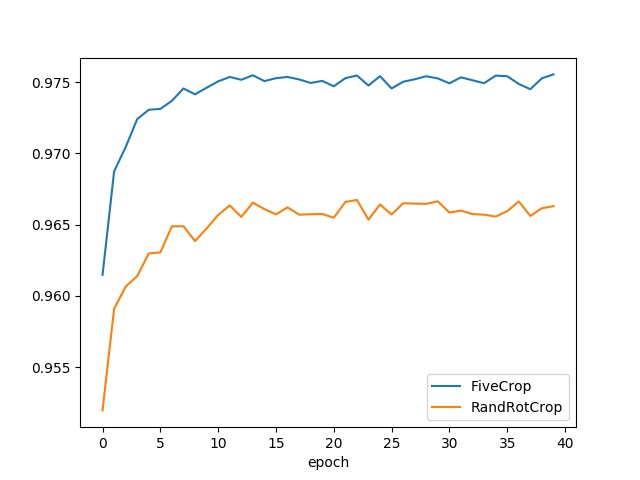
\includegraphics[width=.7\textwidth]{accuracy.jpg}
    \caption{Accuracy over epochs for both data augmentations}
    \label{fig:acc}
\end{figure}

The accuracy does not make sense in this case because there are a disproportionately large number of negative labels in the dataset. For reference, a model that only outputs negative predictions would have gotten a 92.83\% accuracy on the validation set, since accuracy considers true negatives as well. Therefore some other better metric is needed.

\paragraph{Average Precision (AP) Measure:} Instead of accuracy, we can use average precision. We used Scikit-Learn's average precision metrics to calculate the average precision for our model's output.
\begin{itemize}
    \item For FiveCrop augmentation, the best model AP value is: 0.8821
    \item For RandRotCrop augmentation, the best model AP value is: 0.8079
\end{itemize}

Since Five Crop captures information in different parts of the image, it has a broader ``view'' of the image and is hence able to be trained to predict more labels correctly, which results in its AP value being higher. Thus, we use the FiveCrop model in the GUI prediction. We also demonstrate the predictions done by the FiveCrop model for each class in the GUI.
\begin{figure}[H]
    \centering
    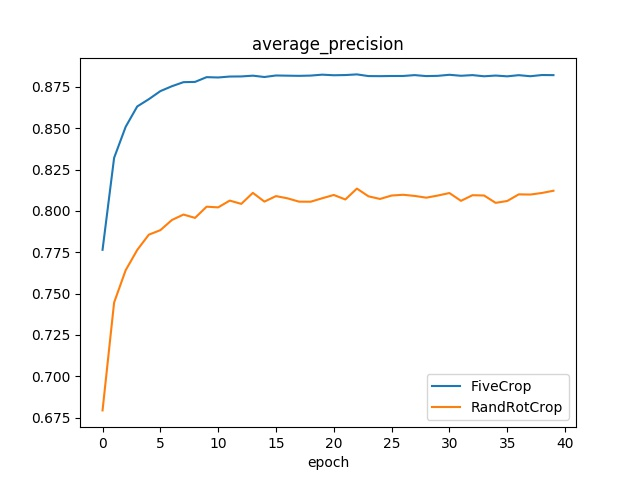
\includegraphics[width=.7\textwidth]{average_precision.jpg}
    \caption{Average precision over epochs for both data augmentations}
    \label{fig:avg_precision}
\end{figure}

\paragraph{Tail Accuracy:}
The demonstrator (GUI) looks good on the top-50 images because images with higher prediction confidence and hence pass the classification threshold, are more likely to be correctly labelled. We can see this in effect in Figure~\ref{fig:tailacc} where the tail accuracy increases along with the classification threshold until they are both close to zero.
\begin{figure}[H]
    \centering
    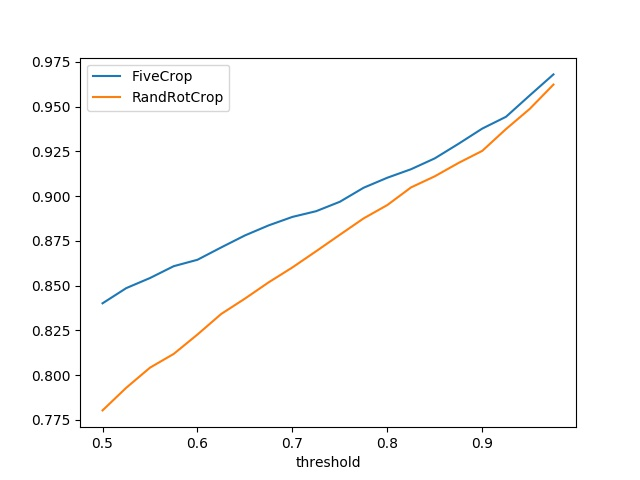
\includegraphics[width=.7\textwidth]{tail_acc.jpg}
    \caption{Average tail accuracy against threshold for both data augmentations}
    \label{fig:tailacc}
\end{figure}

\newpage
\section{Additional Plots}
Here we have the training and validation losses for both FiveCrop and RandRotCrop. The FiveCrop converges to a much lower loss compared to RandRotCrop.
\begin{figure}[H]
    \centering
    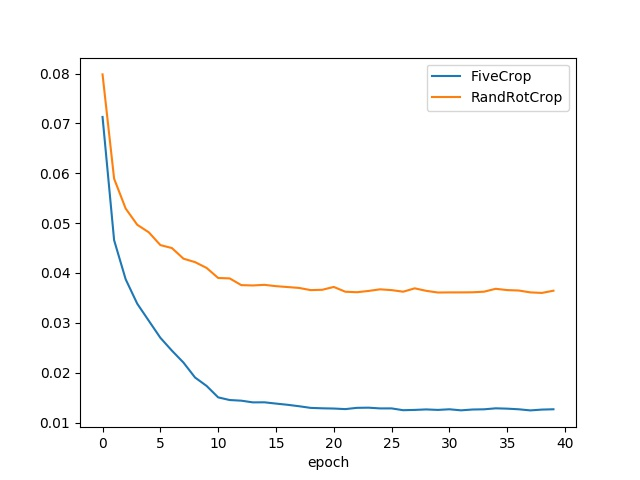
\includegraphics[width=.7\textwidth]{train_loss.jpg}
    \caption{Training loss over epochs for both data augmentations}
    \label{fig:train_loss}
\end{figure}%
\begin{figure}[H]
    \centering
    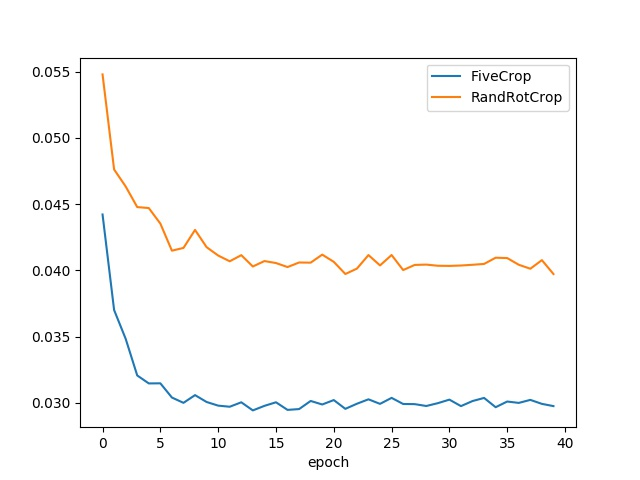
\includegraphics[width=.7\textwidth]{val_loss.jpg}
    \caption{Validation loss over epochs for both data augmentations}
    \label{fig:val_loss}
\end{figure}

\newpage
\section{Instructions}
\subsection{Training and Validation}
There is a need to install Scikit-Learn since we used it to calculate the average precision as well as Pandas since the \url{vocparse.py} code that was provided uses it to parse the VOC dataset. This is of course in addition to both PyTorch and NumPy that is used for deep learning. To install them,
\begin{lstlisting}
$ python -m pip install sklearn pandas torch numpy
\end{lstlisting}

The deep learning code is fairly straightforward. There are two data augmentations. To change the data augmentation, scroll down to the bottom of the Python script \url{pascal.py} and change the \url{FIVE_CROP} variable to whichever you want: \url{True} to use FiveCrop and \url{False} to use RandRotCrop. Assuming the dataset tarfile is in the same directory, we can do the following to run the model training and validation.
\begin{lstlisting}
$ tar -xvf ./VOCtrainval_11-May-2012.tar
$ python pascal.py
\end{lstlisting}

\subsection{Web GUI}
For the web GUI, we will need Flask to act as the backend server, as well as a browser to run the frontend. To install Flask,

\begin{lstlisting}
$ python -m pip install flask
\end{lstlisting}

To get the full experience of the web GUI, you have to unpack the VOC dataset and copy the images to the appropriate folder (for the ranks image preview). The steps for Unix systems are listed below, assuming the dataset tarfile is in the same directory as the Python scripts.
\begin{lstlisting}
$ tar -xvf ./VOCtrainval_11-May-2012.tar
$ cp ./VOCdevkit/VOC2012/JPEGImages/* ./static/images/
$ python app.py
\end{lstlisting}

After running the Python script, open a browser and head to \url{localhost:5000}. You will be greeted by two buttons, one for predict and the other to view the pre-computed top-ranked predictions on the validation set. For the prediction, upload a JPG image and press the predict button. On the other hand, the rankings are separated by class and can be sorted by pressing the table headers.

\paragraph{\textit{Note: Ignore \url{misc.py}, it is used for plotting etc. only}} 
\end{document}


